%!TEX root = main.tex

\subsection {Empirical Study}\label{experiments}
We evaluate ISHA against various baselines,
using Bernoulli arms.
%reward distributions in $\{0,1\}$. 

%We begin by introducing the reservoirs and algorithms.

\textbf{Datasets/reservoirs.}
We test on synthetic data, with arms drawn from various reservoirs.
First, we use $Beta(1,1)$, and $Beta(3,1)$ reservoirs of Equation~\ref{eqn:beta_distribution},
both with support $[0,1]$ and rescaled to have support in $[0.25,0.75]$
to avoid arms with extreme means; these distributions correspond to $\beta=1$ and $\beta=3$ in Equation~\ref{eqn:beta_parameterization}, respectively, regardless of scaling. 
We also use the reservoir described in Equation~\ref{eqn:mostbiasedcoin_reservoir} composed of two spikes with gap $\epsilon$ and relative proportion $\pi$ such that $1/{\pi \epsilon^2}$ is a constant known to govern the sample complexity of this problem \citep{chandrasekaran2014finding,malloy2012quickest,jamieson2016power}.
In particular, the spikes are symmetric around $1/2$ and $(\pi,\epsilon) \in \{(10^{-3},\sqrt{10^{-1}}), (10^{-2},\sqrt{10^{-2}}), (10^{-1},\sqrt{10^{-3}})\}$ so that $1/{\pi \epsilon^2}=10,000$.
% $\epsilon$ is the gap between mean rewards $\mu_1$ and $\mu_2$, where $\alpha$ is the probability of drawing $\mu_1$ and $1-\alpha$ is the probability of drawing $\mu_2$. The mean rewards were centered around $.5$, i.e. $\mu_1 = .5+\frac{\epsilon}{2}$ and $\mu_2 = .5-\frac{\epsilon}{2}$

We also test against a reservoir generated from data collected from the New Yorker Caption Contest dataset~\citep{NIPS2015_5868},
using contest number 637 having 3,795 captions and 875,065 total votes uniformly at random distributed amongst the captions, resulting in about 231 votes per caption. For our experiment, arms are randomly drawn with replacement from the $3,795$ arms, where the mean of each arm is taken to be the fraction of times ``unfunny'' was observed in the dataset, so small means are better. The arm reservoir CDF (Figure~\ref{fig:newyorkercdf}) can be found in Section~\ref{appendix:experiments}.

%% For a more realistic reservoir, we fit a CDF to data from the New
%% Yorker Caption Contest dataset~\citep{NIPS2015_5868,
%%   new_yorker_contest}, contest number 539 having 4,827 captions; data
%% was gathered using the NEXT system~\citep{NIPS2015_5868}.  In each
%% contest, participants are asked to rate proposed captions for cartoons
%% in the New Yorker magazine as funny, somewhat funny, or unfunny.  We
%% use this data to synthesize a reservoir CDF,
%% Figure~\ref{fig:newyorkercdf}, over Bernoulli reward distributions for
%% our experiments.  We treat each caption as an arm, and estimate its
%% expected reward as the number of times it was rated unfunny divided by
%% its total ratings count.

%\paragraph{Algorithms.}
%We use the following algorithms as baselines against Successive Halving with $n^*_T$ arms drawn from the reservoir.
%According to our experiments $n^*_T$ is the optimal or near-optimal choice.
%To demonstrate this point, we also experiment with smaller values of $n$.
%All algorithms in our experiments run for some fixed budget $T$. We experiment with several values of $T$.

%All the algorithms below, apart from \texttt{CBT} and \texttt{Empirical CBT},
%are described for the best arm having the largest mean reward. However, our results are presented in terms of the best arm having the lowest mean.

\textbf{Algorithms.}
We compare against three main
classes of algorithms: (1) pure exploration algorithms, (2)
explore-vs-exploit algorithms, and (3) anytime algorithms.  Detailed
descriptions of these algorithms and their use in our empirical study
are given in Section~\ref{appendix:experiments}.  In brief, within
the pure exploration family, we consider
SIRI~\citep{DBLP:journals/corr/CarpentierV15},
lil'UCB~\citep{Jamieson2014lilU}, Hyperband~\citep{li2017hyperband},
and Successive Rejects~\citep{audibert2010best}.  We also devise a
strong baseline for ISHA that we refer to as Chernoff.
Chernoff has knowledge of $\mu_*$, and simply draws an arm from the
reservoir, tests it so long as its the empirical lower bound does not
exceed $\mu_*$, discarding the arm and drawing another if the arm is
ever proven to be suboptimal.  Within the explore-vs-exploit family,
we consider four infinite-armed bandit algorithms of \cite{berry1997}, CBT
and Empirical CBT \citep{Chan2018Infinite}, and fixed horizon Two
Target \citep{bonald2013two}.  We also consider an anytime version of ISHA:
choose increasing dyadic numbers of arms, $n=2^i, i=1,2,\dots$.  For each value of $n$,
sample $n$ new arms and run ISHA and save the result as the best arm found so far.  We compare this
algorithm to Hyperband Anytime and SIRI Anytime (using the budget
doubling trick as proposed by the SIRI authors).

\subsubsection{Experiments and Insights}\label{fb-experiments}
Our proposed algorithm starts discarding arms after just a single pull, far before concentration of measure has kicked in. 
%Empirical studies of Hyperband which hedges over parallel versions of Successive Halving where each has the same budget but different number of arms have anecdotally shown that the most aggressive bracket with the most arms, tends to be the superior bracket \citep{li2017hyperband}. 
It is truly surprising that theoretical results can be obtained for such a result, and consequently we begin with an empirical study of this phenomenon. 
We evaluate ISHA against a variety of alternative approaches. Our exhaustive experiments can be found in Section~\ref{appendix:experiments}, here we report only a representative sample.
% Here we present two types of experiments:
% (1) finding the ``right'' number of arms for Successive Halving such that simple regret is minimized, and
% (2) evaluating the simple regret of Successive Halving vs. the baselines described above for various values of budget $T$.

\textbf{Successive Halving performance as a function of the number of arms for a fixed budget.}
Figure~\ref{fig:sh-num-arms:alpha1_beta3_scaled} studies the tradeoff between the number of arms $n$ and budget $T$ for Successive Halving in terms of simple regret averaged over 500 replications. Let $n^*_T$ be the maximum number of arms in Successive Halving,
i.e. $T \geq n^*_T \log_2 n^*_T$.
Each ``sheet'' of the plot corresponds to a single value of budget $T$ for a number of arms $n=2,2^2,2^3,\dots,n^*_T$.
We observe that across a variety of reservoirs (see Section~\ref{appendix:experiments}) Successive Halving with the maximum possible number of arms $n^*_T$ (ISHA) appears to perform better than or as well as Successive Halving with any other value of $n$.

% Choosing the optimal number of arms is the main variable in deciding how to optimally run Successive Halving in the infinite setting.
% A given reservoir will have some minimum number of arms necessary to
% obtain a ``good'' arm with sufficient probability;
% this effect is especially noticeable for the Two Spike reservoirs.
% For each reservoir, we observe better
% performance on average for a given budget as the number of arms is
% increased, provided the budget is sufficient to obtain any ``good'' arms.
% However, even when the budget is too small to obtain a ``good'' arm the
% performance never degrades by increasing the number of arms.

% We conjecture that given the choice between drawing more arms (with fewer pulls per arms in each round) or fewer arms (with more pulls per arm in each round), the former is either the optimal choice or a good choice (i.e. does not result in significant additional regret) for Successive Halving when nothing is known about the reservoir.
% In short, $n^*_T$ arms is always a good choice for Successive Halving in the infinite setting.

% Next, we test our algorithm against some baselines.
\textbf{Simple regret vs. Budget.} 
In the next several plots we compare the simple regret of
ISHA to that of various baselines. The results are averaged over 200 replications.
In Figures~\ref{fig:sh-infinite:alpha1_beta3_scaled}
and \ref{fig:sh-infinite:TwoSpike_1}
we compare to state-of-the-art algorithms for infinitely-armed bandit models. 
While different algorithms are most competitive on different reservoirs, ISHA and Successive Rejects are the only algorithms that are consistently superior across all reservoirs.
%See Appendix~\ref{appendix:experiments} for the results on all other reservoirs.
% We added Empirical CBT, a regret algorithm, due to its adaptability to unknown reservoirs.
% We also include Successive Rejects, a finite bandit algorithm, with the
% same number of arms that Successive Halving uses.
% Note that SIRI (known $\beta$) is only run on beta distributions as it requires knowledge of $\beta$. Successive Halving almost always beats its natural competitors SIRI and Hyperband. Empirical CBT sometimes performs better than Successive Halving, but not consistently or dramatically. This makes the point that when nothing is known about the reservoir distribution, Successive Halving is a safe choice.

% The performance of Successive Halving and Successive Rejects are consistently similar, regardless of the
% reservoir distribution.
% This is not surprising, as the two algorithms are similar.
% In particular, Successive Rejects will also throw out arms based on a
% single sample when run with $n^*_T$ arms.
 
Figure~\ref{fig:sh-lilucb:alpha1_beta3_scaled} highlights, as discussed in some detail in Section~\ref{intro}, the difficulty of
choosing the optimal number of arms for UCB-style algorithms,
such as the lil'UCB.
%Appendix~\ref{appendix:experiments} for similar results on more reservoirs.

Figure~\ref{fig:sh-unscaled-alpha1_beta1_unscaled} compares mainly against exploration-vs-exploitation baselines.
Recall that many of these baseline algorithms are designed specifically for $Beta$ reservoirs and assume knowledge of
of the reservoir. Even so, ISHA does as well or better. 
%See Appendix~\ref{appendix:experiments} for a second similar result.


Finally, in Figure~\ref{fig:sh-anytime:alpha1_beta3_scaled}, we compare ISHA 
and ISHA Anytime to several other anytime algorithms.
%These algorithms are designed to use an arbitrarily large budget and iteratively refine their notion of the best arm available in such
%a way that they eventually converge on the optimal arm.
ISHA Anytime easily outperforms its baselines,
performing nearly as well as its non-Anytime version. 
%See Appendix~\ref{appendix:experiments} for similar results on more reservoirs.

​​​​​\begin{figure}
\centering
\begin{subfigure}{0.325\textwidth}%
	\includegraphics[width=\textwidth]{fixedbudget/figures/folder1/alpha1_beta3_scaled.png}
	\centering
	\caption{$Beta(3,1)$ Scaled.}
	\label{fig:sh-num-arms:alpha1_beta3_scaled}
\end{subfigure}
\begin{subfigure}{0.325\textwidth}%
	\includegraphics[width=\textwidth]{fixedbudget/figures/folder4/alpha1_beta3_scaled.png}
	\caption{$Beta(3,1)$ Scaled}
	\label{fig:sh-infinite:alpha1_beta3_scaled}
\end{subfigure}
\begin{subfigure}{0.325\textwidth}
	\includegraphics[width=\textwidth]{fixedbudget/figures/folder4/{TwoSpike_0.1_0.515_0.031}.png}
	\caption{Spikes $\pi=10^{-1}, \epsilon=\sqrt{10^{-3}}$}
	\label{fig:sh-infinite:TwoSpike_1}
\end{subfigure}
\begin{subfigure}{0.325\textwidth}%
	\includegraphics[width=\textwidth]{fixedbudget/figures/folder5/alpha1_beta3_scaled.png}
	\caption{$Beta(3,1)$ Scaled}
	\label{fig:sh-lilucb:alpha1_beta3_scaled}
\end{subfigure}
\begin{subfigure}{0.325\textwidth}%
	\includegraphics[width=\textwidth]{fixedbudget/figures/folder3/alpha1_beta3_scaled.png}
	\caption{$Beta(3,1)$ Scaled}
	\label{fig:sh-anytime:alpha1_beta3_scaled}
\end{subfigure}
\begin{subfigure}{0.325\textwidth}%
	\includegraphics[width=\textwidth]{fixedbudget/figures/folder2/alpha1_beta1_unscaled.png}
	\caption{$Beta(1,1)$ }
	\label{fig:sh-unscaled-alpha1_beta1_unscaled}
\end{subfigure}
\caption{A sampled set of results. See Section~\ref{appendix:experiments} for more.}
\end{figure}

%\begin{figure}
%\centering
%\caption{Impact of the number of arms for a fixed budget and reservoir.}
%\begin{subfigure}{0.4\textwidth}
%	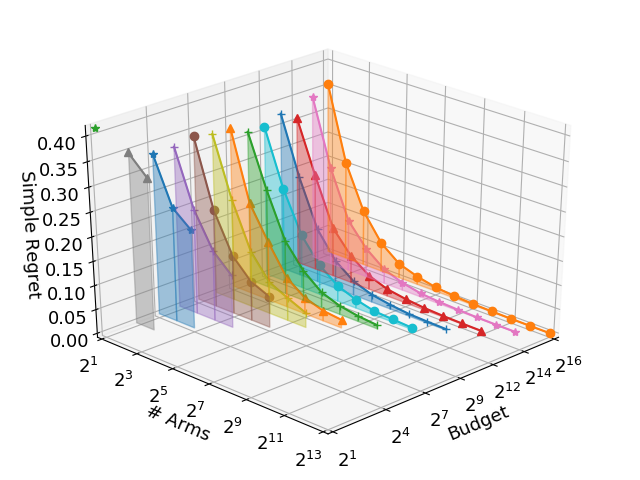
\includegraphics[width=\textwidth]{figures/folder1/alpha1_beta1_unscaled.png}
%	\caption{$Beta(1,1)$}
%	\label{fig:sh-num-arms:alpha1_beta1_unscaled}
%\end{subfigure}
%\quad
%\begin{subfigure}{0.4\textwidth}
%	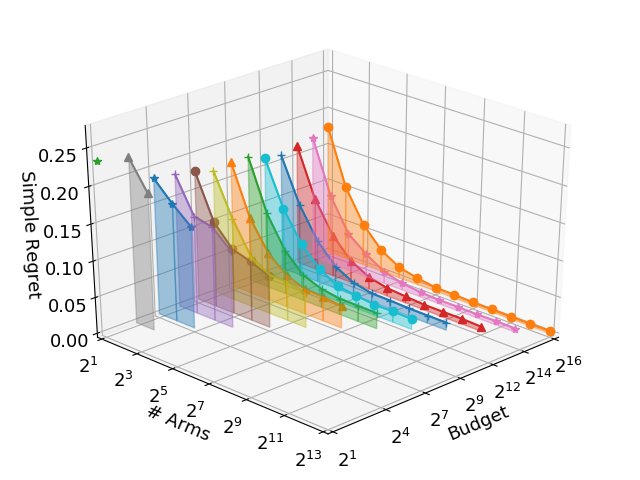
\includegraphics[width=\textwidth]{figures/folder1/alpha1_beta1_scaled.png}
%	\caption{$Beta(1,1)$ Scaled}
%	\label{fig:sh-num-arms:alpha1_beta1_scaled}
%\end{subfigure}
%%
%\begin{subfigure}{0.4\textwidth}
%	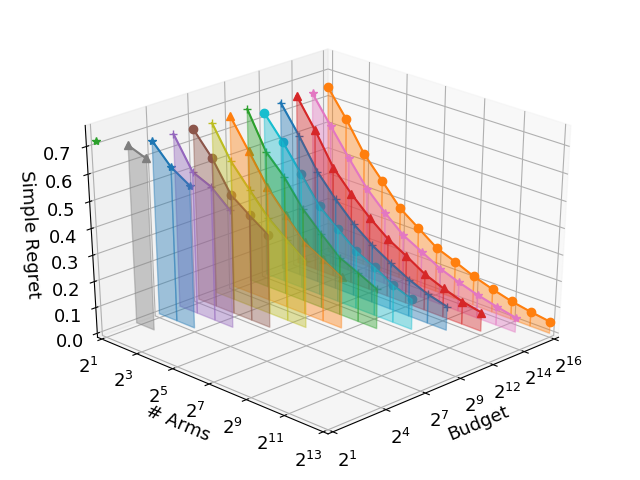
\includegraphics[width=\textwidth]{figures/folder1/alpha1_beta3_unscaled.png}
%	\caption{$Beta(3,1)$}
%	\label{fig:sh-num-arms:alpha1_beta3_unscaled}
%\end{subfigure}
%\quad
%\begin{subfigure}{0.4\textwidth}
%	\includegraphics[width=\textwidth]{figures/folder1/alpha1_beta3_scaled.png}
%	\caption{$Beta(3,1)$ Scaled}
%	\label{fig:sh-num-arms:alpha1_beta3_scaled}
%\end{subfigure}
%%
%\begin{subfigure}{0.4\textwidth}
%	\includegraphics[width=\textwidth]{figures/folder1/{TwoSpike_0.1_0.515_0.031}.png}
%	\caption{TwoSpike $\alpha=0.1, \epsilon=\sqrt{0.001}$}
%	\label{fig:sh-num-arms:TwoSpike_1}
%\end{subfigure}
%\quad
%\begin{subfigure}{0.4\textwidth}
%	\includegraphics[width=\textwidth]{figures/folder1/{TwoSpike_0.01_0.55_0.1}.png}
%	\caption{Two Spike $\alpha=0.01, \epsilon=\sqrt{0.01}$}
%	\label{fig:sh-num-arms:TwoSpike_2}
%\end{subfigure}
%%
%\begin{subfigure}{0.4\textwidth}
%	\includegraphics[width=\textwidth]{figures/folder1/{TwoSpike_0.001_0.658_0.316}.png}
%	\caption{Two Spike $\alpha=0.001, \epsilon=\sqrt{0.1}$}
%	\label{fig:sh-num-arms:TwoSpike_3}
%\end{subfigure}
%\quad
%\begin{subfigure}{0.4\textwidth}
%	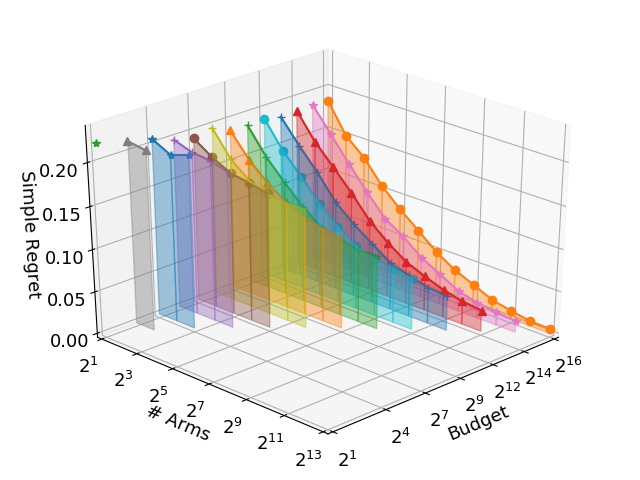
\includegraphics[width=\textwidth]{figures/folder1/new_yorker.png}
%	\caption{New Yorker}
%	\label{fig:sh-num-arms:new_yorker}
%\end{subfigure}
%\label{fig:sh-num-arms}
%\end{figure}
%
%\begin{figure}
%\centering
%\caption{Comparison to state-of-the-art pure exploration infinite bandit algorithms}
%\begin{subfigure}{0.4\textwidth}
%	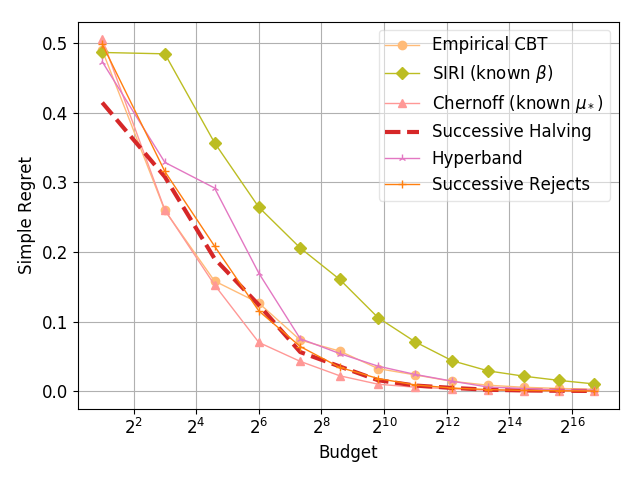
\includegraphics[width=\textwidth]{figures/folder4/alpha1_beta1_unscaled.png}
%	\caption{$Beta(1,1)$}
%	\label{fig:sh-infinite:alpha1_beta1_unscaled}
%\end{subfigure}
%\quad
%\begin{subfigure}{0.4\textwidth}
%	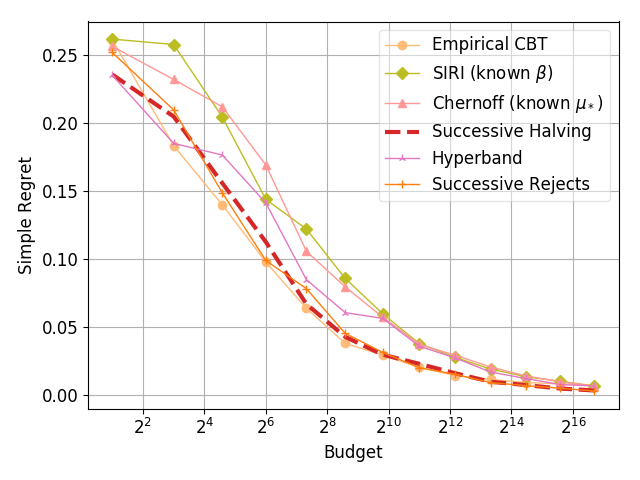
\includegraphics[width=\textwidth]{figures/folder4/alpha1_beta1_scaled.png}
%	\caption{$Beta(1,1)$ Scaled}
%	\label{fig:sh-infinite:alpha1_beta1_scaled}
%\end{subfigure}
%%
%\begin{subfigure}{0.4\textwidth}
%	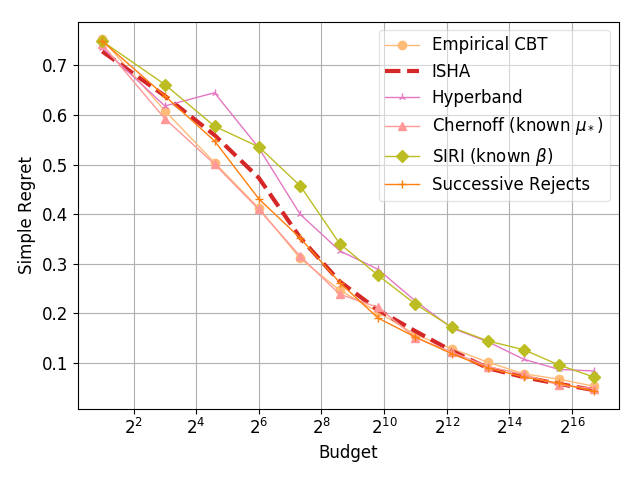
\includegraphics[width=\textwidth]{figures/folder4/alpha1_beta3_unscaled.png}
%	\caption{$Beta(3,1)$}
%	\label{fig:sh-infinite:alpha1_beta3_unscaled}
%\end{subfigure}
%\quad
%\begin{subfigure}{0.4\textwidth}
%	\includegraphics[width=\textwidth]{figures/folder4/alpha1_beta3_scaled.png}
%	\caption{$Beta(3,1)$ Scaled}
%	\label{fig:sh-infinite:alpha1_beta3_scaled}
%\end{subfigure}
%%
%\begin{subfigure}{0.4\textwidth}
%	\includegraphics[width=\textwidth]{figures/folder4/{TwoSpike_0.1_0.515_0.031}.png}
%	\caption{TwoSpike $\alpha=0.1, \epsilon=\sqrt{0.001}$}
%	\label{fig:sh-infinite:TwoSpike_1}
%\end{subfigure}
%\quad
%\begin{subfigure}{0.4\textwidth}
%	\includegraphics[width=\textwidth]{figures/folder4/{TwoSpike_0.01_0.55_0.1}.png}
%	\caption{Two Spike $\alpha=0.01, \epsilon=\sqrt{0.01}$}
%	\label{fig:sh-infinite:TwoSpike_2}
%\end{subfigure}
%%
%\begin{subfigure}{0.4\textwidth}
%	\includegraphics[width=\textwidth]{figures/folder4/{TwoSpike_0.001_0.658_0.316}.png}
%	\caption{Two Spike $\alpha=0.001, \epsilon=\sqrt{0.1}$}
%	\label{fig:sh-infinite:TwoSpike_3}
%\end{subfigure}
%\quad
%\begin{subfigure}{0.4\textwidth}
%	\includegraphics[width=\textwidth]{figures/folder4/new_yorker.png}
%	\caption{New Yorker}
%	\label{fig:sh-infinite:new_yorker}
%\end{subfigure}
%\label{fig:sh-infinite}
%\end{figure}
%
%
%\begin{figure}
%\centering
%\caption{Comparison to lil'UCB}
%\begin{subfigure}{0.4\textwidth}
%	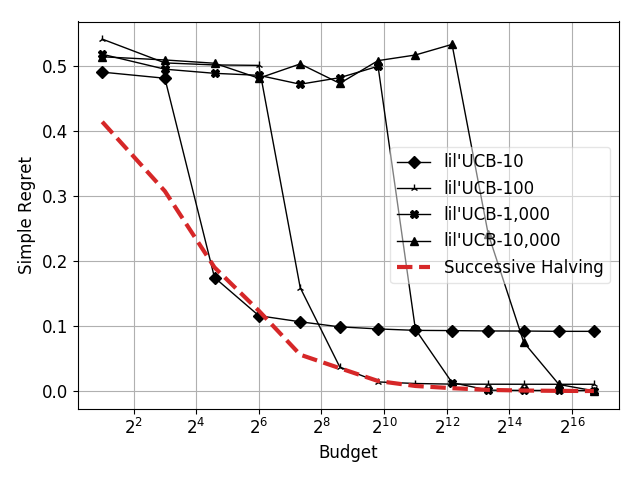
\includegraphics[width=\textwidth]{figures/folder5/alpha1_beta1_unscaled.png}
%	\caption{$Beta(1,1)$}
%	\label{fig:sh-lilucb:alpha1_beta1_unscaled}
%\end{subfigure}
%\quad
%\begin{subfigure}{0.4\textwidth}
%	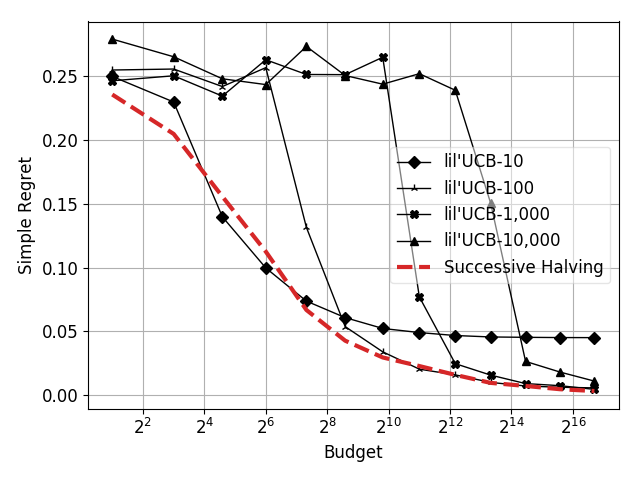
\includegraphics[width=\textwidth]{figures/folder5/alpha1_beta1_scaled.png}
%	\caption{$Beta(1,1)$ Scaled}
%	\label{fig:sh-lilucb:alpha1_beta1_scaled}
%\end{subfigure}
%%
%\begin{subfigure}{0.4\textwidth}
%	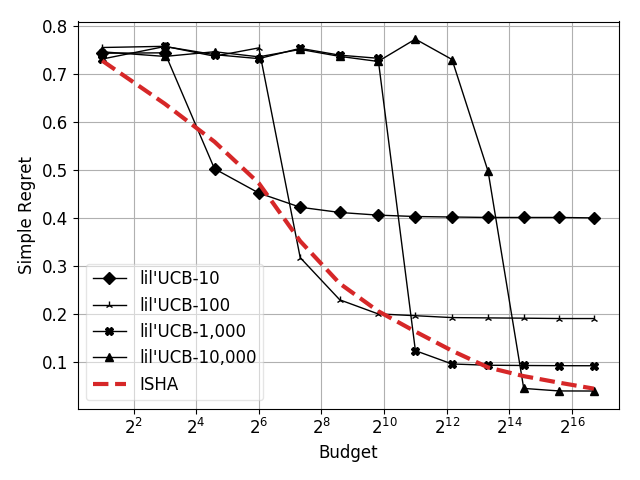
\includegraphics[width=\textwidth]{figures/folder5/alpha1_beta3_unscaled.png}
%	\caption{$Beta(3,1)$}
%	\label{fig:sh-lilucb:alpha1_beta3_unscaled}
%\end{subfigure}
%\quad
%\begin{subfigure}{0.4\textwidth}
%	\includegraphics[width=\textwidth]{figures/folder5/alpha1_beta3_scaled.png}
%	\caption{$Beta(3,1)$ Scaled}
%	\label{fig:sh-lilucb:alpha1_beta3_scaled}
%\end{subfigure}
%%
%%\begin{subfigure}{0.4\textwidth}
%%	\includegraphics[width=\textwidth]{figures/folder5/new_yorker.png}
%%	\caption{New Yorker}
%%	\label{fig:sh-lilucb:new_yorker}
%%\end{subfigure}
%\label{fig:sh-lilucb}
%\end{figure}
%
%
%\begin{figure}
%\centering
%\caption{Comparison to state-of-the-art explore-vs-exploit infinite bandit algorithms}
%\begin{subfigure}{0.4\textwidth}
%	\includegraphics[width=\textwidth]{figures/folder2/alpha1_beta1_unscaled.png}
%	\caption{$Beta(1,1)$}
%	\label{fig:sh-unscaled-alpha1_beta1_unscaled}
%\end{subfigure}
%\quad
%\begin{subfigure}{0.4\textwidth}
%	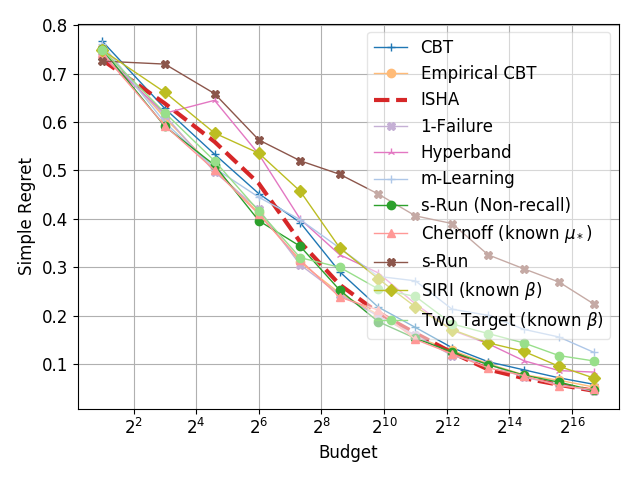
\includegraphics[width=\textwidth]{figures/folder2/alpha1_beta3_unscaled.png}
%	\caption{$Beta(3,1)$}
%	\label{fig:sh-unscaled-alpha1_beta3_unscaled}
%\end{subfigure}
%\label{fig:sh-unscaled}
%\end{figure}
%
%
%\begin{figure}
%\centering
%\caption{Anytime Performance}
%\begin{subfigure}{0.4\textwidth}
%	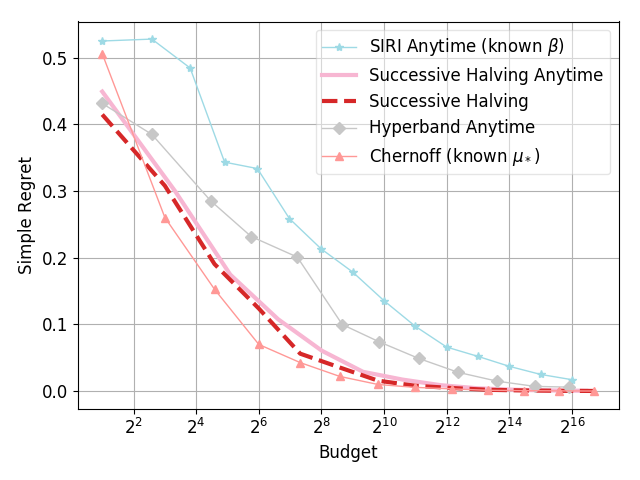
\includegraphics[width=\textwidth]{figures/folder3/alpha1_beta1_unscaled.png}
%	\caption{$Beta(1,1)$}
%	\label{fig:sh-anytime:alpha1_beta1_unscaled}
%\end{subfigure}
%\quad
%\begin{subfigure}{0.4\textwidth}
%	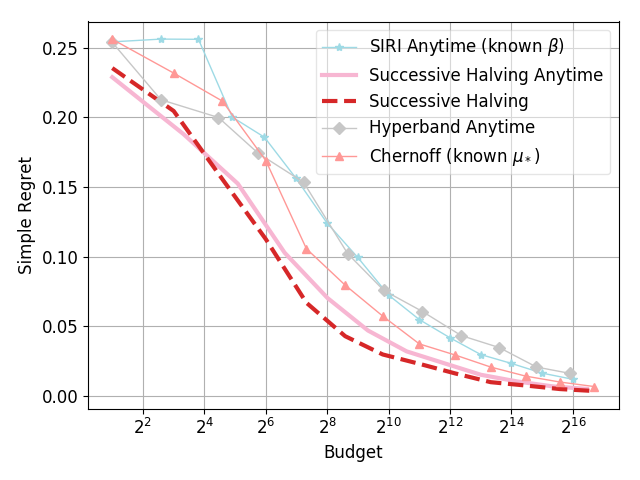
\includegraphics[width=\textwidth]{figures/folder3/alpha1_beta1_scaled.png}
%	\caption{$Beta(1,1)$ Scaled}
%	\label{fig:sh-anytime:alpha1_beta1_scaled}
%\end{subfigure}
%%
%\begin{subfigure}{0.4\textwidth}
%	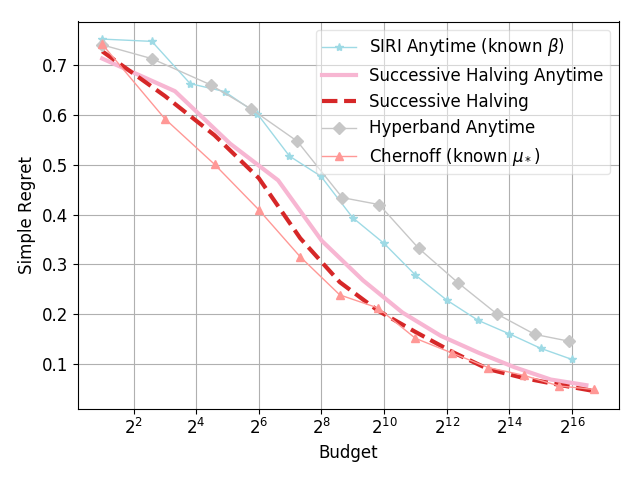
\includegraphics[width=\textwidth]{figures/folder3/alpha1_beta3_unscaled.png}
%	\caption{$Beta(3,1)$}
%	\label{fig:sh-anytime:alpha1_beta3_unscaled}
%\end{subfigure}
%\quad
%\begin{subfigure}{0.4\textwidth}
%	\includegraphics[width=\textwidth]{figures/folder3/alpha1_beta3_scaled.png}
%	\caption{$Beta(3,1)$ Scaled}
%	\label{fig:sh-anytime:alpha1_beta3_scaled}
%\end{subfigure}
%%
%\label{fig:sh-anytime}
%\end{figure}
